\documentclass[]{article}
\usepackage[top=1.3in,bottom=1.3in,left=1in,right=1in]{geometry}
\usepackage{tikz}
\usetikzlibrary{shapes.geometric,arrows.meta}
\usepackage{subcaption}
\usepackage{xcolor}
\usepackage[colorlinks,allcolors=blue]{hyperref}
\usepackage[noabbrev]{cleveref}


\title{
    {\LARGE Rules for the Game of}
    \\[1ex]
    {\Huge\bf RoPaSci~360}
}
\author{
    COMP30024 Artificial Intelligence
%     \textbf{Matthew Farrugia-Roberts}
%     \\
%     \textit{The University of Melbourne}
%     \\
%     \href
%       {mailto:matt.farrugia@unimelb.edu.au}
%       {\tt matt.farrugia@unimelb.edu.au}
}
\date{2021}


% Custom TikZ commands
\newcommand{\hex}[4] {
    \node[hex,fill={#3}] at ({#1}, {#2}) {};
    \node[hex,thick,draw={#3},fill={#3!10}] at ({#1}, {#2}) {};
    \node at ({#1}, {#2}) {{#4}};
}
\newcommand{\uptoken}[3] {
    \node[draw,circle,minimum size=6.8mm,fill=white] at (#1, #2) {};
    \node[draw,circle,minimum size=5.2mm,very thick,black]  at (#1, #2) {};
    \node[] at (#1, #2) {#3};
}
\newcommand{\lotoken}[3] {
    \node[draw,circle,minimum size=6.8mm,fill=white] at (#1, #2) {};
    \node[draw,circle,minimum size=5.2mm,very thick,purple] at (#1, #2) {};
    \node[] at (#1, #2) {#3};
}

\newcommand{\board} {
    \tikzset{
        hex/.style={
            regular polygon,
            regular polygon sides=6,
            minimum size=10mm,
            inner sep=0mm,
            outer sep=0mm,
            rotate=30,
            draw
        },
        x={(4.33mm,7.5mm)},
        y={(8.66mm,0mm)}
    }
    \foreach \r/\q in {
                    +4/-4,+4/-3,+4/-2,+4/-1,+4/+0,
                 +3/-4,+3/-3,+3/-2,+3/-1,+3/+0,+3/+1,
              +2/-4,+2/-3,+2/-2,+2/-1,+2/+0,+2/+1,+2/+2,
           +1/-4,+1/-3,+1/-2,+1/-1,+1/+0,+1/+1,+1/+2,+1/+3,
        +0/-4,+0/-3,+0/-2,+0/-1,+0/+0,+0/+1,+0/+2,+0/+3,+0/+4,
           -1/-3,-1/-2,-1/-1,-1/+0,-1/+1,-1/+2,-1/+3,-1/+4,
              -2/-2,-2/-1,-2/+0,-2/+1,-2/+2,-2/+3,-2/+4,
                 -3/-1,-3/+0,-3/+1,-3/+2,-3/+3,-3/+4,
                    -4/+0,-4/+1,-4/+2,-4/+3,-4/+4,
    }
        \node[hex,fill=black!5] at (\r, \q) {};
}

\begin{document}

\maketitle

\begin{quote}
    \emph{RoPaSci~360} is a simultaneous-play board game of chance and
    anticipation in the spirit of the storied hand-game known by many
    names throughout the world, including \emph{Roshambo}, \emph{Jan-Ken},
    and, of course, \emph{Rock-Paper-Scissors}.
    Throw down a team of tokens with which to crush, cover, and cut
    through your opponent.
    Attack them when and where they least expect it, but be quick to
    slip away or you won't escape their retaliation!
    Have you anticipated your opponent's next move,
    or are you thinking exactly what they want you to think?
    \emph{Rock, paper, scissors, throw!}
\end{quote}

\section*{Overview}

\emph{RoPaSci~360} is played on a hexagonal \textbf{board} of
61~\textbf{hexes}, which may be \textbf{occupied} by \textbf{tokens}.
%
Each token has one of 3~\textbf{symbols}: \textbf{Rock}, \textbf{Paper}, or
\textbf{Scissors}.
%
Two \textbf{players} (named \textbf{Upper} and \textbf{Lower}) play the game.
%
The game begins with an empty board, but throughout the game, each player
will \textbf{throw} up to 9 tokens onto the board
(for example, see \Cref{fig:example}).
%
The goal of each player is to catch and \textbf{defeat} their opponent's
tokens, as per the mechanic of \emph{Rock-Paper-Scissors} (\Cref{fig:rps}).

\begin{figure}[ht!]
\centering
\begin{subfigure}{.38\textwidth}
    \centering
    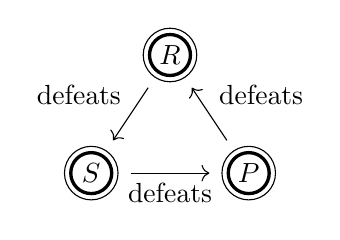
\begin{tikzpicture}
        \uptoken{+1.0}{+1.5}{$R$}
        \uptoken{+2.0}{+0.0}{$P$}
        \uptoken{+0.0}{+0.0}{$S$}
        \begin{scope}[every path/.style={
                shorten >=5mm,
                shorten <=5mm,
                -{>[length=1mm]}
            }]
            \draw (1.0, 1.5) -- node[above left]  {defeats} (0.0, 0.0);
            \draw (0.0, 0.0) -- node[below]       {defeats} (2.0, 0.0);
            \draw (2.0, 0.0) -- node[above right] {defeats} (1.0, 1.5);
        \end{scope}
    \end{tikzpicture}
    \caption{\label{fig:rps} (above)
        Rock-Paper-Scissors mechanic:
        Rock defeats Scissors,
        Scissors defeats Paper, and
        Paper defeats Rock.
    }
    \caption{
        \label{fig:example} (right)
        Four turns into this example game, Upper has thrown three
        tokens onto the board:
        One Rock ($R$), one Paper ($P$), and one Scissors ($S$).
        Upper has six throws remaining.
        Lower has five throws remaining, having thrown one Paper ($p$),
        one Scissors ($s$), and two Rocks ($r_1, r_2$).
        So far no tokens have been defeated, but $S$ should watch out for
        $r_2$, it's only two hexes away!
    }
\end{subfigure}
\begin{subfigure}{.01\textwidth}\end{subfigure}
\begin{subfigure}{.60\textwidth}
    \centering
    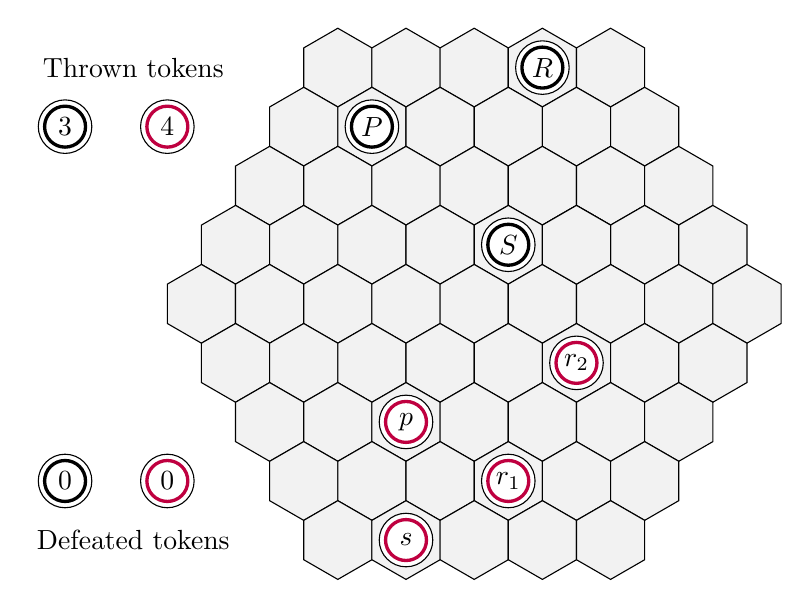
\begin{tikzpicture}
        \board
        % upper
        \uptoken{+4}{-1}{$R$}
        \uptoken{+3}{-3}{$P$}
        \uptoken{+1}{+0}{$S$}
        % lower
        \lotoken{-1}{+2}{$r_2$}
        \lotoken{-2}{+0}{$p$}
        \lotoken{-3}{+2}{$r_1$}
        \lotoken{-4}{+1}{$s$}
        % throws
        \node[] at (+4, -7.0) {Thrown tokens};
        \uptoken   {+3}{-7.5} {3}
        \lotoken   {+3}{-6.0} {4}
        % defeats
        \uptoken   {-3}{-4.5} {0}
        \lotoken   {-3}{-3.0} {0}
        \node[] at (-4, -3.0) {Defeated tokens};
    \end{tikzpicture}
\end{subfigure}
\caption{
    The core Rock-Paper-Scissors mechanic, and an example game configuration.
    More details below.
}
\end{figure}

\newpage

\section*{Gameplay}

The game proceeds in turns. In each turn, both players take an
\textbf{action}.
%
Both actions are chosen and taken \emph{at the same time}.
%
Each action might be a \textbf{throw action}, a \textbf{slide action},
or a \textbf{swing action}.
%
Afterwards, if there are any \textbf{overlapping tokens}
(groups of multiple tokens occupying one hex), these tokens \textbf{battle}.
%
These turns continue until the game ends.
%
The rules for each type of action, along with the rules for battling
overlapping tokens and ending the game, are described below.

\subsection*{Throw actions}

In a \textbf{throw action} (a `throw'), a player adds a single new token,
with a symbol of their choice (Rock, Paper, or Scissors), to the board.
% 
Each player can take the throw action \emph{at most 9~times per game}.
%
When throwing their $n$\textsuperscript{th} token since the start of the
game, the player can choose any hex from the first $n$ rows of hexes for
this new token.
Upper counts from the top row down, and Lower counts from the bottom row
up (see \Cref{fig:throwzones}).
%
The chosen hex may be empty or may already be occupied by another token of
either player.

\subsection*{Slide actions}

In a \textbf{slide action} (a `slide'), a player moves an existing token from
the hex it currently occupies to an \textbf{adjacent hex}
    (one of the at-most-six hexes in direct contact with the current
    hex---see \Cref{fig:slide}).
%
The adjacent hex may be empty or may already be occupied by another token of
either player.

\subsection*{Swing actions}

In a \textbf{swing action} (a `swing'), a player moves an existing token from
the hex it currently occupies \emph{around} an adjacent \textbf{swinging hex}
to an \textbf{opposite hex}. Opposite hexes are those adjacent to the swinging
hex but not adjacent to the current hex, and not the current hex itself
(see \Cref{fig:swing}).
%
The swinging hex \emph{must be occupied by at least one of the player's
tokens}---tokens cannot swing around empty hexes or hexes occupied only
by opponent tokens.
%
The opposite hex may be empty occupied by other tokens of either player.

\begin{figure}[ht!]
\centering
\begin{subfigure}{.37\textwidth}
    \centering
    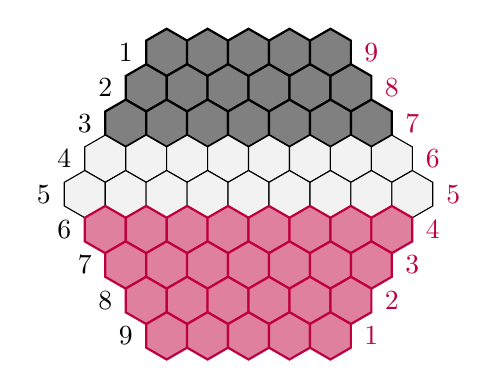
\begin{tikzpicture}
    \tikzset{
        hex/.style={regular polygon,regular polygon sides=6,draw,rotate=30,
            minimum size=6mm,inner sep=0mm,outer sep=0mm,},
        x={(2.60mm,4.5mm)},
        y={(5.20mm,0mm)}
    }
    \foreach \r/\q in {
                    +4/-4,+4/-3,+4/-2,+4/-1,+4/+0,
                 +3/-4,+3/-3,+3/-2,+3/-1,+3/+0,+3/+1,
              +2/-4,+2/-3,+2/-2,+2/-1,+2/+0,+2/+1,+2/+2
    }
        \node[hex,fill=black!50,draw,thick] at (\r, \q) {};
    \foreach \r/\q in {
           +1/-4,+1/-3,+1/-2,+1/-1,+1/+0,+1/+1,+1/+2,+1/+3,
        +0/-4,+0/-3,+0/-2,+0/-1,+0/+0,+0/+1,+0/+2,+0/+3,+0/+4
    }
        \node[hex,fill=black!5] at (\r, \q) {};
    \foreach \r/\q in {
           -1/-3,-1/-2,-1/-1,-1/+0,-1/+1,-1/+2,-1/+3,-1/+4,
              -2/-2,-2/-1,-2/+0,-2/+1,-2/+2,-2/+3,-2/+4,
                 -3/-1,-3/+0,-3/+1,-3/+2,-3/+3,-3/+4,
                    -4/+0,-4/+1,-4/+2,-4/+3,-4/+4
    }
        \node[hex,fill=purple!50,thick,draw=purple] at (\r, \q) {};
    % counters
    \node at (+4, -5) {1};
    \node at (+3, -5) {2};
    \node at (+2, -5) {3};
    \node at (+1, -5) {4};
    \node at (+0, -5) {5};
    \node at (-1, -4) {6};
    \node at (-2, -3) {7};
    \node at (-3, -2) {8};
    \node at (-4, -1) {9};
    \node at (+4, +1) {\color{purple}9};
    \node at (+3, +2) {\color{purple}8};
    \node at (+2, +3) {\color{purple}7};
    \node at (+1, +4) {\color{purple}6};
    \node at (+0, +5) {\color{purple}5};
    \node at (-1, +5) {\color{purple}4};
    \node at (-2, +5) {\color{purple}3};
    \node at (-3, +5) {\color{purple}2};
    \node at (-4, +5) {\color{purple}1};
    \end{tikzpicture}
    \caption{
        \label{fig:throwzones}
        On Upper's third \textbf{throw}, Upper selects a hex from the top
        three hex rows (coloured black, all rows numbered on left).
        %
        On Lower's fourth throw, Lower selects a hex from the bottom
        four hex rows (coloured {\color{purple}purple}, numbered right).
    }
\end{subfigure}
\begin{subfigure}{.01\textwidth}\end{subfigure}
\begin{subfigure}{.27\textwidth}
    \centering
    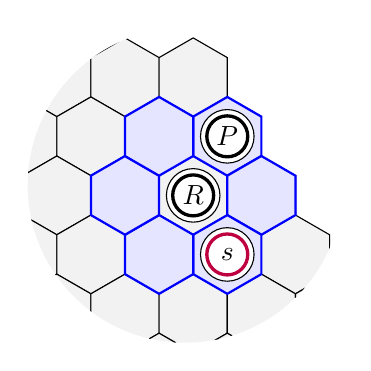
\begin{tikzpicture}
        \clip (1.63,1.63) circle (2);
        \board
        \hex{+3}{+1}{blue}{}
        \hex{+2}{+2}{blue}{}
        \hex{+1}{+2}{blue}{}
        \hex{+1}{+1}{blue}{}
        \hex{+2}{+0}{blue}{}
        \hex{+3}{+0}{blue}{}
        \uptoken{+2}{+1}{$R$}
        \uptoken{+3}{+1}{$P$}
        \lotoken{+1}{+2}{$s$}
    \end{tikzpicture}
    \caption{\label{fig:slide}
        The six hexes \textbf{adjacent} to $R$'s hex are marked in
        {\color{blue}blue}.
        $R$ can \textbf{slide} to any of these hexes, including those
        already occupied by $P$ and $s$.
        $P$'s hex is only adjacent to \emph{four} hexes, since it's near
        an edge of the board.
    }
\end{subfigure}
\begin{subfigure}{.01\textwidth}\end{subfigure}
\begin{subfigure}{.32\textwidth}
    \centering
    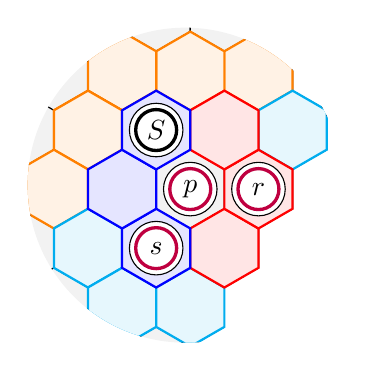
\begin{tikzpicture}
        \clip (2.1,-0.7) circle (2);
        \board
        \hex{+1}{+3}{orange}{}
        \hex{+1}{+2}{orange}{}
        \hex{+1}{+1}{orange}{}
        \hex{+0}{+1}{orange}{}
        \hex{+0}{+1}{orange}{}
        \hex{-1}{+1}{orange}{}
        \hex{+0}{+4}{cyan}{}
        \hex{-2}{+2}{cyan}{}
        \hex{-3}{+3}{cyan}{}
        \hex{-3}{+4}{cyan}{}
        \hex{-2}{+4}{red}{}
        \hex{-1}{+4}{red}{}
        \hex{+0}{+3}{red}{}
        \hex{-2}{+3}{blue}{}
        \hex{-1}{+2}{blue}{}
        \hex{+0}{+2}{blue}{}
        \lotoken{-1}{+4}{$r$}
        \lotoken{-1}{+3}{$p$}
        \lotoken{-2}{+3}{$s$}
        \uptoken{+0}{+2}{$S$}
    \end{tikzpicture}
    \caption{\label{fig:swing}
        Lower's $r$ can \textbf{swing} (around $p$'s hex) to the hexes on
        the \emph{opposite side} of $p$ ({\color{blue}blue}), but \emph{not}
        to the hexes on the \emph{same side} ({\color{red}red}).
        Lower's $p$ can swing around $r$'s or $s$'s hexes (to
        {\color{cyan}cyan} hexes), but \emph{not} around hexes without
        Lower tokens (to {\color{orange}orange} hexes).
    }
\end{subfigure}
\caption{
    On each turn, both players simultaneously choose a throw action,
    a slide action, or a swing action.
}
\end{figure}

\newpage

\subsection*{Overlapping tokens}

After every action, there may be hexes occupied by more than one token,
of one or both players.
%
These tokens \textbf{battle} according to the Rock-Paper-Scissors mechanic,
with \textbf{defeated} tokens removed from the board:
%
\begin{itemize}
    \item
        If the hex is occupied by one or more tokens with each symbol,
        \emph{all of the tokens are defeated.}
    \item
        If the hex is occupied by a Rock token, all Scissors tokens there are
        defeated.
    \item
        If the hex is occupied by a Scissors token, all Paper tokens there are
        defeated.
    \item
        If the hex is occupied by a Paper token, all Rock tokens there are
        defeated.
\end{itemize}
%
Even tokens controlled by a single player will battle if they share a hex.
%
Moreover, a hex might remain occupied by multiple tokens if all of these
tokens have the same symbol.
%
See \Cref{fig:battles} for further clarification.

\section*{Ending the game}

The game ends when one of the following conditions is met
(if multiple are met, use the first in this list).

\begin{enumerate}
    \item
        One player has no remaining throws and all of their tokens have
        been defeated:
        If the other player still has tokens or throws, declare that player
        the \textbf{winner}.
        Otherwise, declare a \textbf{draw}.
    \item
        A token is \textbf{invincible} if it cannot be defeated by the
        opponent's remaining tokens, and the opponent has no remaining
        throws.
        Both players have an invincible token: Declare a \textbf{draw}
        (see \Cref{fig:draw}).
    \item
        One player has an invincible token (see condition 2) and the
        other has only one remaining token (not invincible):
        Declare the player with the invincible token the \textbf{winner}
        (see \Cref{fig:winner}).
        % also it seems to make sense that a player has to actually make
        % a winning throw in order to win so maybe the remaining throws
        % should not automatically make a player win, right?
    \item
        One game configuration (with the same number of tokens with each
        symbol and controlling player occupying each hex, and the same
        number of throws remaining for each player),
        occurs for a third time since the start of the game
        (not necessarily in succession):
        Declare a \textbf{draw}.
    \item
        The players have had their 360\textsuperscript{th} turn without a
        winner being declared:
        Declare a \textbf{draw}.
\end{enumerate}

\begin{figure}[ht!]
\centering
\begin{subfigure}{.32\textwidth}
    \centering
    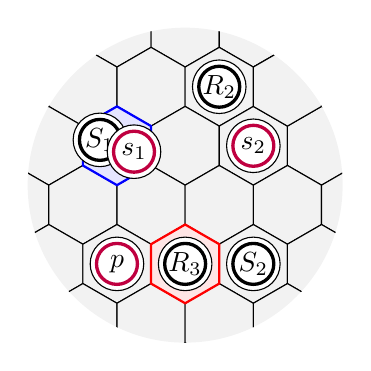
\begin{tikzpicture}
        \clip (0.0,-0.5) circle (2);
        \board
        % clash
        \hex{+0}{-1}{blue}{}
        \uptoken{+0.1}{-1.3}{$S_1$}
        \lotoken{-0.1}{-0.7}{$s_1$}
        % all three
        \hex{-2}{+1}{red}{}
        \lotoken{-2}{+0}{$p$}
        \uptoken{-2}{+1}{$R_3$}
        \uptoken{-2}{+2}{$S_2$}
        % two more
        \uptoken{+1}{+0}{$R_2$}
        \lotoken{+0}{+1}{$s_2$}
    \end{tikzpicture}
    \caption{
        \label{fig:battles}
        Two Scissors tokens remain undefeated on the {\color{blue}blue}
        hex.
        %
        If $p$ and $S_2$ slide onto the {\color{red}red} hex, $R_3$, $p$,
        and $S_2$ will \textit{all} be defeated.
        %
        If $p$ slides onto the {\color{red}red} hex but $R_2$ slides onto
        $s_2$'s hex, then $R_3$ and $s_2$ will be defeated.
    }
\end{subfigure}
\begin{subfigure}{.01\textwidth}\end{subfigure}
\begin{subfigure}{.32\textwidth}
    \centering
    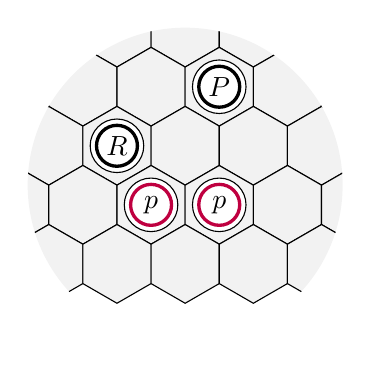
\begin{tikzpicture}
        \clip (0,-2.0) circle (2);
        \board
        \lotoken{-3}{+1}{$p$}
        \lotoken{-3}{+2}{$p$}
        \uptoken{-1}{+1}{$P$}
        \uptoken{-2}{+0}{$R$}
    \end{tikzpicture}
    \caption{\label{fig:draw}
        If neither player has throws or Scissors tokens remaining,
        and both players have Paper tokens remaining, these
        Paper tokens are invincible.
        The second end-of-game condition is met, so the game is declared
        a draw.
    }
\end{subfigure}
\begin{subfigure}{.01\textwidth}\end{subfigure}
\begin{subfigure}{.32\textwidth}
    \centering
    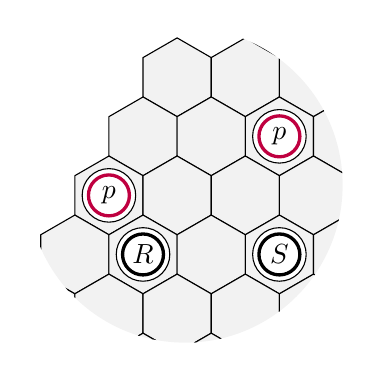
\begin{tikzpicture}
        \clip (-1.63,1.63) circle (2);
        \board
        \lotoken{+2}{-4}{$p$}
        \lotoken{+3}{-2}{$p$}
        \uptoken{+1}{-1}{$S$}
        \uptoken{+1}{-3}{$R$}
    \end{tikzpicture}
    \caption{\label{fig:winner}
        If Lower has only Paper tokens, and no throws remaining, then Upper's
        Scissors token is invincible.
        If Upper can defeat either of Lower's remaining Paper tokens, we will
        declare Upper the winner by condition 3.
    }
\end{subfigure}
\caption{
    In these examples, assume all tokens are visible, and neither
    player has remaining throws.
}
\end{figure}

\end{document}
